\section{Sampled inference results}
\label{sec:followup}
\subsection{Accuracy across output limits}
Trace checkpoints averaged 80.21\% accuracy at 2K, compared with 67.97\% for the unchanged student, a descriptive difference of +12.24 percentage points. The corresponding differences at 4K and 8K were -1.30 and -1.30 points (Table~\ref{tab:followup-accuracy}).
\par\begin{table}[ht]\centering\small\begin{tabular}{llrrr}\toprule
Checkpoint & Training seed & 2K (\%) & 4K (\%) & 8K (\%) \\
\midrule
Unchanged & -- & 67.97 & 85.94 & 87.50 \\
Teacher trace & 42 & 80.47 & 82.81 & 86.72 \\
Teacher trace & 43 & 82.03 & 83.59 & 85.94 \\
Teacher trace & 44 & 78.12 & 87.50 & 85.94 \\
Trace mean & -- & 80.21 & 84.64 & 86.20 \\
Trace mean $-$ unchanged & -- & +12.24 & -1.30 & -1.30 \\
\bottomrule\end{tabular}\caption{Numerical primary accuracy on the same 128 questions at each output limit. The trace mean averages three trained checkpoints; the last row gives percentage-point differences. Thinking-mode sampling uses one fixed decoding seed and effective batches of 32/16/8.}\label{tab:followup-accuracy}\end{table}\par
At the follow-up's primary 8K limit, trace checkpoints averaged 86.20\% versus 87.50\% unchanged. The mean difference was -1.30 percentage points (95\% paired item-bootstrap interval -5.73 to +2.86); the training-seed difference SD was 0.45 points. The interval conditions on the three trained checkpoints and the one decoding seed. The 8K numerical comparison establishes neither an accuracy advantage nor equivalence. Comparisons at 2K/4K are descriptive.
\par\begin{figure}[ht]\centering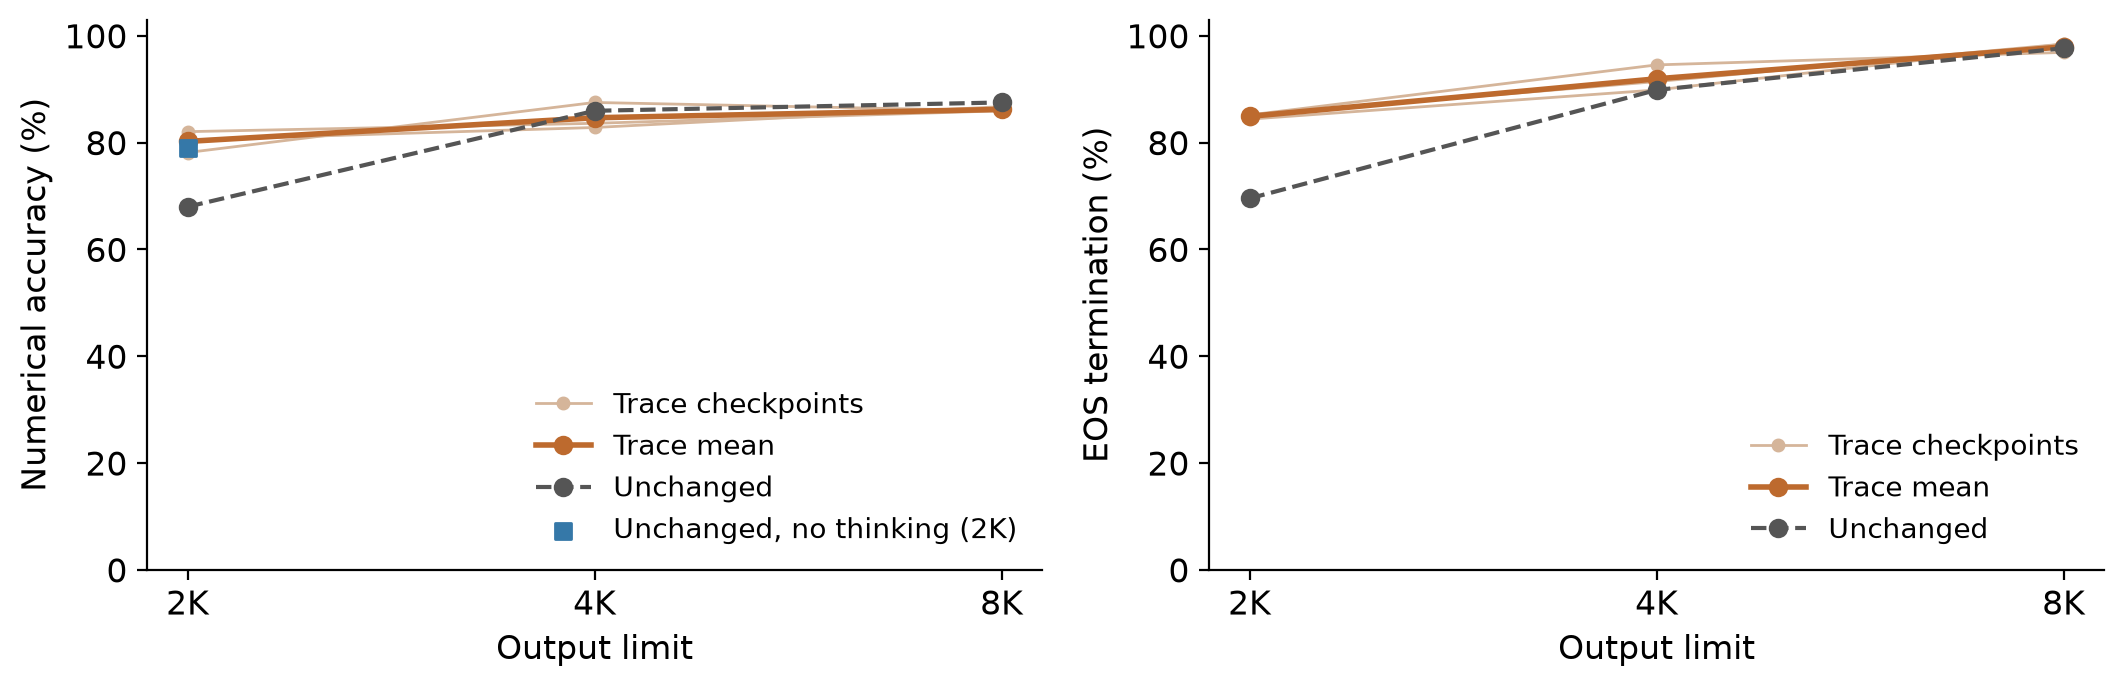
\includegraphics[width=\textwidth]{assets/inference-extension-2026-10-20.png}
\caption{Sampled follow-up on 128 shared questions. Left: numerical accuracy; the blue square is the unchanged student's sampled no-thinking policy, tested only at 2K. Right: fraction terminating at EOS rather than the output limit. Thin orange lines are individual trace checkpoints; thicker lines show their mean. Effective batch size changes with the limit.}\label{fig:followup}\end{figure}\par
\subsection{Sensitivity to final-answer formatting}
Five unchanged-student responses at 8K contain repeated, numerically consistent correct boxes. They pass the numerical primary rule and fail the exactly-one-box secondary rule. The trace scores are unchanged. The strict rule therefore reverses the point estimate to +2.60 points, with a conditional item interval of -2.60 to +8.07 (Table~\ref{tab:format-sensitivity}). Neither rule establishes an 8K advantage. The primary rule was fixed before the follow-up generations and is retained throughout.
\par\begin{table}[ht]\centering\small\begin{tabular}{lrrr}\toprule
8K scoring rule & Unchanged (\%) & Trace mean (\%) & Difference (pp) \\
\midrule
Numerical, primary & 87.50 & 86.20 & -1.30 \\
One box, secondary & 83.59 & 86.20 & +2.60 \\
\bottomrule\end{tabular}\caption{The same 128 questions and raw generations, scored under two prospectively retained rules. The numerical primary accepts repeated identical numeric boxes; the strict secondary requires exactly one box. Differences are trace mean minus unchanged.}\label{tab:format-sensitivity}\end{table}\par
\subsection{Completion and response length}
At 2K, 69.53\% of unchanged-student responses ended at an end-of-sequence (EOS) token, compared with 84.90\% across trace checkpoints. Mean generated lengths were 1451 and 994 tokens, respectively. At 8K, EOS rates were 97.66\% and 97.92\%; trace checkpoints still generated fewer tokens on average (1520 versus 2012; Table~\ref{tab:followup-completion}). These lengths include all generated thinking and final-response tokens, subject to the stated limits.
\par\begin{table}[ht]\centering\small\begin{tabular}{llrrrr}\toprule
Checkpoint & Seed & Correct/128 & EOS (\%) & Unfinished (\%) & Tokens \\
\midrule
Unchanged & -- & 112 & 97.66 & 2.34 & 2012 \\
Teacher trace & 42 & 111 & 98.44 & 1.56 & 1511 \\
Teacher trace & 43 & 110 & 98.44 & 1.56 & 1575 \\
Teacher trace & 44 & 110 & 96.88 & 3.12 & 1473 \\
\bottomrule\end{tabular}\caption{Completion and mean generated tokens at 8K. Unfinished denotes an unclosed thinking block, which is distinct from EOS termination. Missing or invalid final fields remain incorrect.}\label{tab:followup-completion}\end{table}\par
\subsection{Native no-thinking inference and the failed training control}
Disabling the unchanged student's thinking channel yielded 77.34\% accuracy with greedy decoding and 78.91\% with its recommended sampled policy. The original answer-only checkpoints averaged 6.51\% under greedy decoding on these exact 128 questions. Native no-thinking therefore did not reproduce the answer-only SFT collapse (Table~\ref{tab:nothinking}). Both native no-thinking runs terminated at EOS on all 128 questions.
\par\begin{table}[ht]\centering\small\begin{tabular}{llrr}\toprule
Checkpoint or recipe & Decoding & Accuracy (\%) & Mean tokens \\
\midrule
Unchanged, no thinking & greedy & 77.34 & 239 \\
Unchanged, no thinking & sampled & 78.91 & 237 \\
Unchanged, thinking & greedy & 74.22 & 1386 \\
Answer-only SFT, seed 42 & greedy & 5.47 & 12 \\
Answer-only SFT, seed 43 & greedy & 7.03 & 11 \\
Answer-only SFT, seed 44 & greedy & 7.03 & 11 \\
\bottomrule\end{tabular}\caption{All entries use the same 128 questions at 2K. Greedy thinking and answer-only entries are retained original outputs on this subset, not reruns. The no-thinking sampled policy uses temperature 0.7 and top-p 0.8; it must not be treated as decoder-matched to greedy outputs.}\label{tab:nothinking}\end{table}\par
The sampled native policy used 237 mean tokens, compared with 994 for trace checkpoints at 2K, with accuracies of 78.91\% and 80.21\%. This is a descriptive comparison of complete inference recipes: thinking and no-thinking use different sampling parameters. Disabling the explicit thinking channel also permits worked steps in the final response; it does not imply an absence of reasoning.
